\section{Prior Investigations to this Problem}

\begin{spacing}{2.0}

    The accepted concept of ion pairing that is widely cited today came from the work of Fuoss \cite{P-JACS-1954-v76-Sadek} and Winstein 
    \cite{P-JACS-1956-v78-Winstein} during the 1950s. Before their work, the solvent was usually modeled as a part of the continuum model, where 
    the solvent's electrostatic influence was treated as one single entity, which gave rise to a two-state model. One of those two states being 
    the associated states, where the ions are held close together by their electrostatic interactions, and another state being the dissociated 
    state, where the ions are separated far enough to not attracting each other again. However, Fuoss and Winstein showed in their work that 
    there exists another state that lies in between the dissociated and the associated states of the ions. Therefore, the state in between shall 
    not have the ions too separated that they do not see another's attraction, but not too close that the association is mainly the electrostatic 
    interaction between the ions. For this reason, the state in between could be thought of as another associated state with some influence from 
    the solvent. In this document, we will call this state the solvent separated ion pair (SSIP), and the associated state the contacted ion pair 
    (CIP) for convenience. We also provide a summary illustration of the concept below,

    \begin{equation}
        \underset{\text{free ions}}{\mathrm{M}^+ + \mathrm{X}^-\vphantom{p}} \iff
        \underset{\text{SSIP}}{\mathrm{M} \cdots \mathrm{X}\vphantom{p}} \iff
        \underset{\text{CIP}}{\mathrm{M} \cdot \mathrm{X}\vphantom{p}}
        \label{eq:c1s1-ionpairillus}
    \end{equation} 

    The earliest simulation that attempted to study this type of reaction came from the work of Belch et al. in 1986. \cite{P-JACS-1986-v108-Belch} 
    Although the work did not compute the free energy, it was among the first attempts to analyze the behavior of the solvent through computer 
    simulations. Belch et al. proposed that for a solution of NaCl in water, the Na+ cation tries to maintain the octahedral structure in the CIP 
    state, the SSIP state, and the dissociated state. The work also pointed out that as the dissociation takes place, one water molecule would 
    rotate to form a bridge between the two ions and the hydrogen bond structure between water molecules in the first and the second solvation 
    shells become disrupted. It is evident from this result that the solvent plays a role in the dissociation of CIP. However, how the solvent 
    plays the role in this process still remained a mystery at that point.

    The thermodynamics and the kinetics model of this type of reaction would not complete without the free energy landscape and the information 
    of the free energy barrier between the SSIP and the CIP states. For any simulations performed under the canonical ensemble (fixed numbers of 
    particles, volume, and temperature), the relative Helmholtz free energy can be computed by just taking a natural logarithm of the probability 
    of finding a particular configuration of the ensemble,

    \begin{equation}
        A(\mathbf{x}) = -k_B T \ln\mathbb{P}(\mathbf{x})
    \end{equation}

    \noindent where $k_B$ is the Boltzmann's constant, and $T$ is the temperature of the simulation. Since a collective variable $\xi(\mathbf{x})$
    is also a function of the Cartesian coordinates in the phase space, the Helmholtz free energy could also be computed in terms of the collective
    variable through the following relationship,

    \begin{equation}
        A\left(\xi(\mathbf{x})\right) = -k_B T \ln\int\delta\left(\xi(\mathbf{x}') - \xi(\mathbf{x})\right)e^{V(\mathbf{x})/k_B T} d\mathbf{x}'
    \end{equation}

    Initial attempts on free energy landscape computation began from a very simple model of 1 collective variable chosen from an intuitive guess. 
    Since we hope to study the association / dissociation of the ions, the most natural collective variable that would serve the purpose would be 
    $r_{+-}$. Hence, the relative Helmholtz free energy based on this collective variable would allow us to quantitatively determine the free 
    energy barrier that separates the SSIP state from the CIP state. Numerous works have since published the one-dimensional free energy landscapes 
    in $r_{+-}$, most of which allowed both qualitative and quantitative distinctions between the SSIP and CIP states as two separate metastable 
    states. [CITE 1D WORKS] For group 1 cations, Fennell et al. published detailed comparisons of the free energy trend down the same group. 
    \cite{P-JPhysChemB-2009-v113}. He found that the CIP structure of LiCl has a very steep well of about XX kcal/mol, whereas the CIP free energy 
    barrier of CsCl is very shallow, and for CsCl, the CIP structure is even less thermodynamically stable than the SSIP structure. 

    Although the free energy of ion pairing in aqueous solutions in terms of $r_{+-}$ can give us a rough idea of the SSIP and the CIP behaviors 
    of the system, it does not capture the dynamics of the solvent as hinted by Belch et al. \cite{P-JACS-1986-v108-Belch}, which was confirmed 
    by the later work of Geissler et al. \cite{P-JPhysChemB-1999-v103-Geissler}. In the work of Geissler et al., they employed transition path 
    sampling to characterize the behavior at the transition state [CHECK], and found that there are many probable transition pathways where 
    collective motion of solvent molecules play an important role. A subsequent work by Ballard and Dellago also pointed out that using only 
    $r_{+-}$ as a hypothetical reaction coordinate for this process is inherently a bad choice. \cite{P-JPhysChemB-2012-v116-Ballard} They also 
    found that the influence of the solvent for the NaCl reaction extends up to the third shell, consistent with what was found by Belch et al. 
    \cite{P-JACS-1986-v108-Belch}

    % TEST ADDING A FIGURE
    \begin{figure}[H]
        \centering
        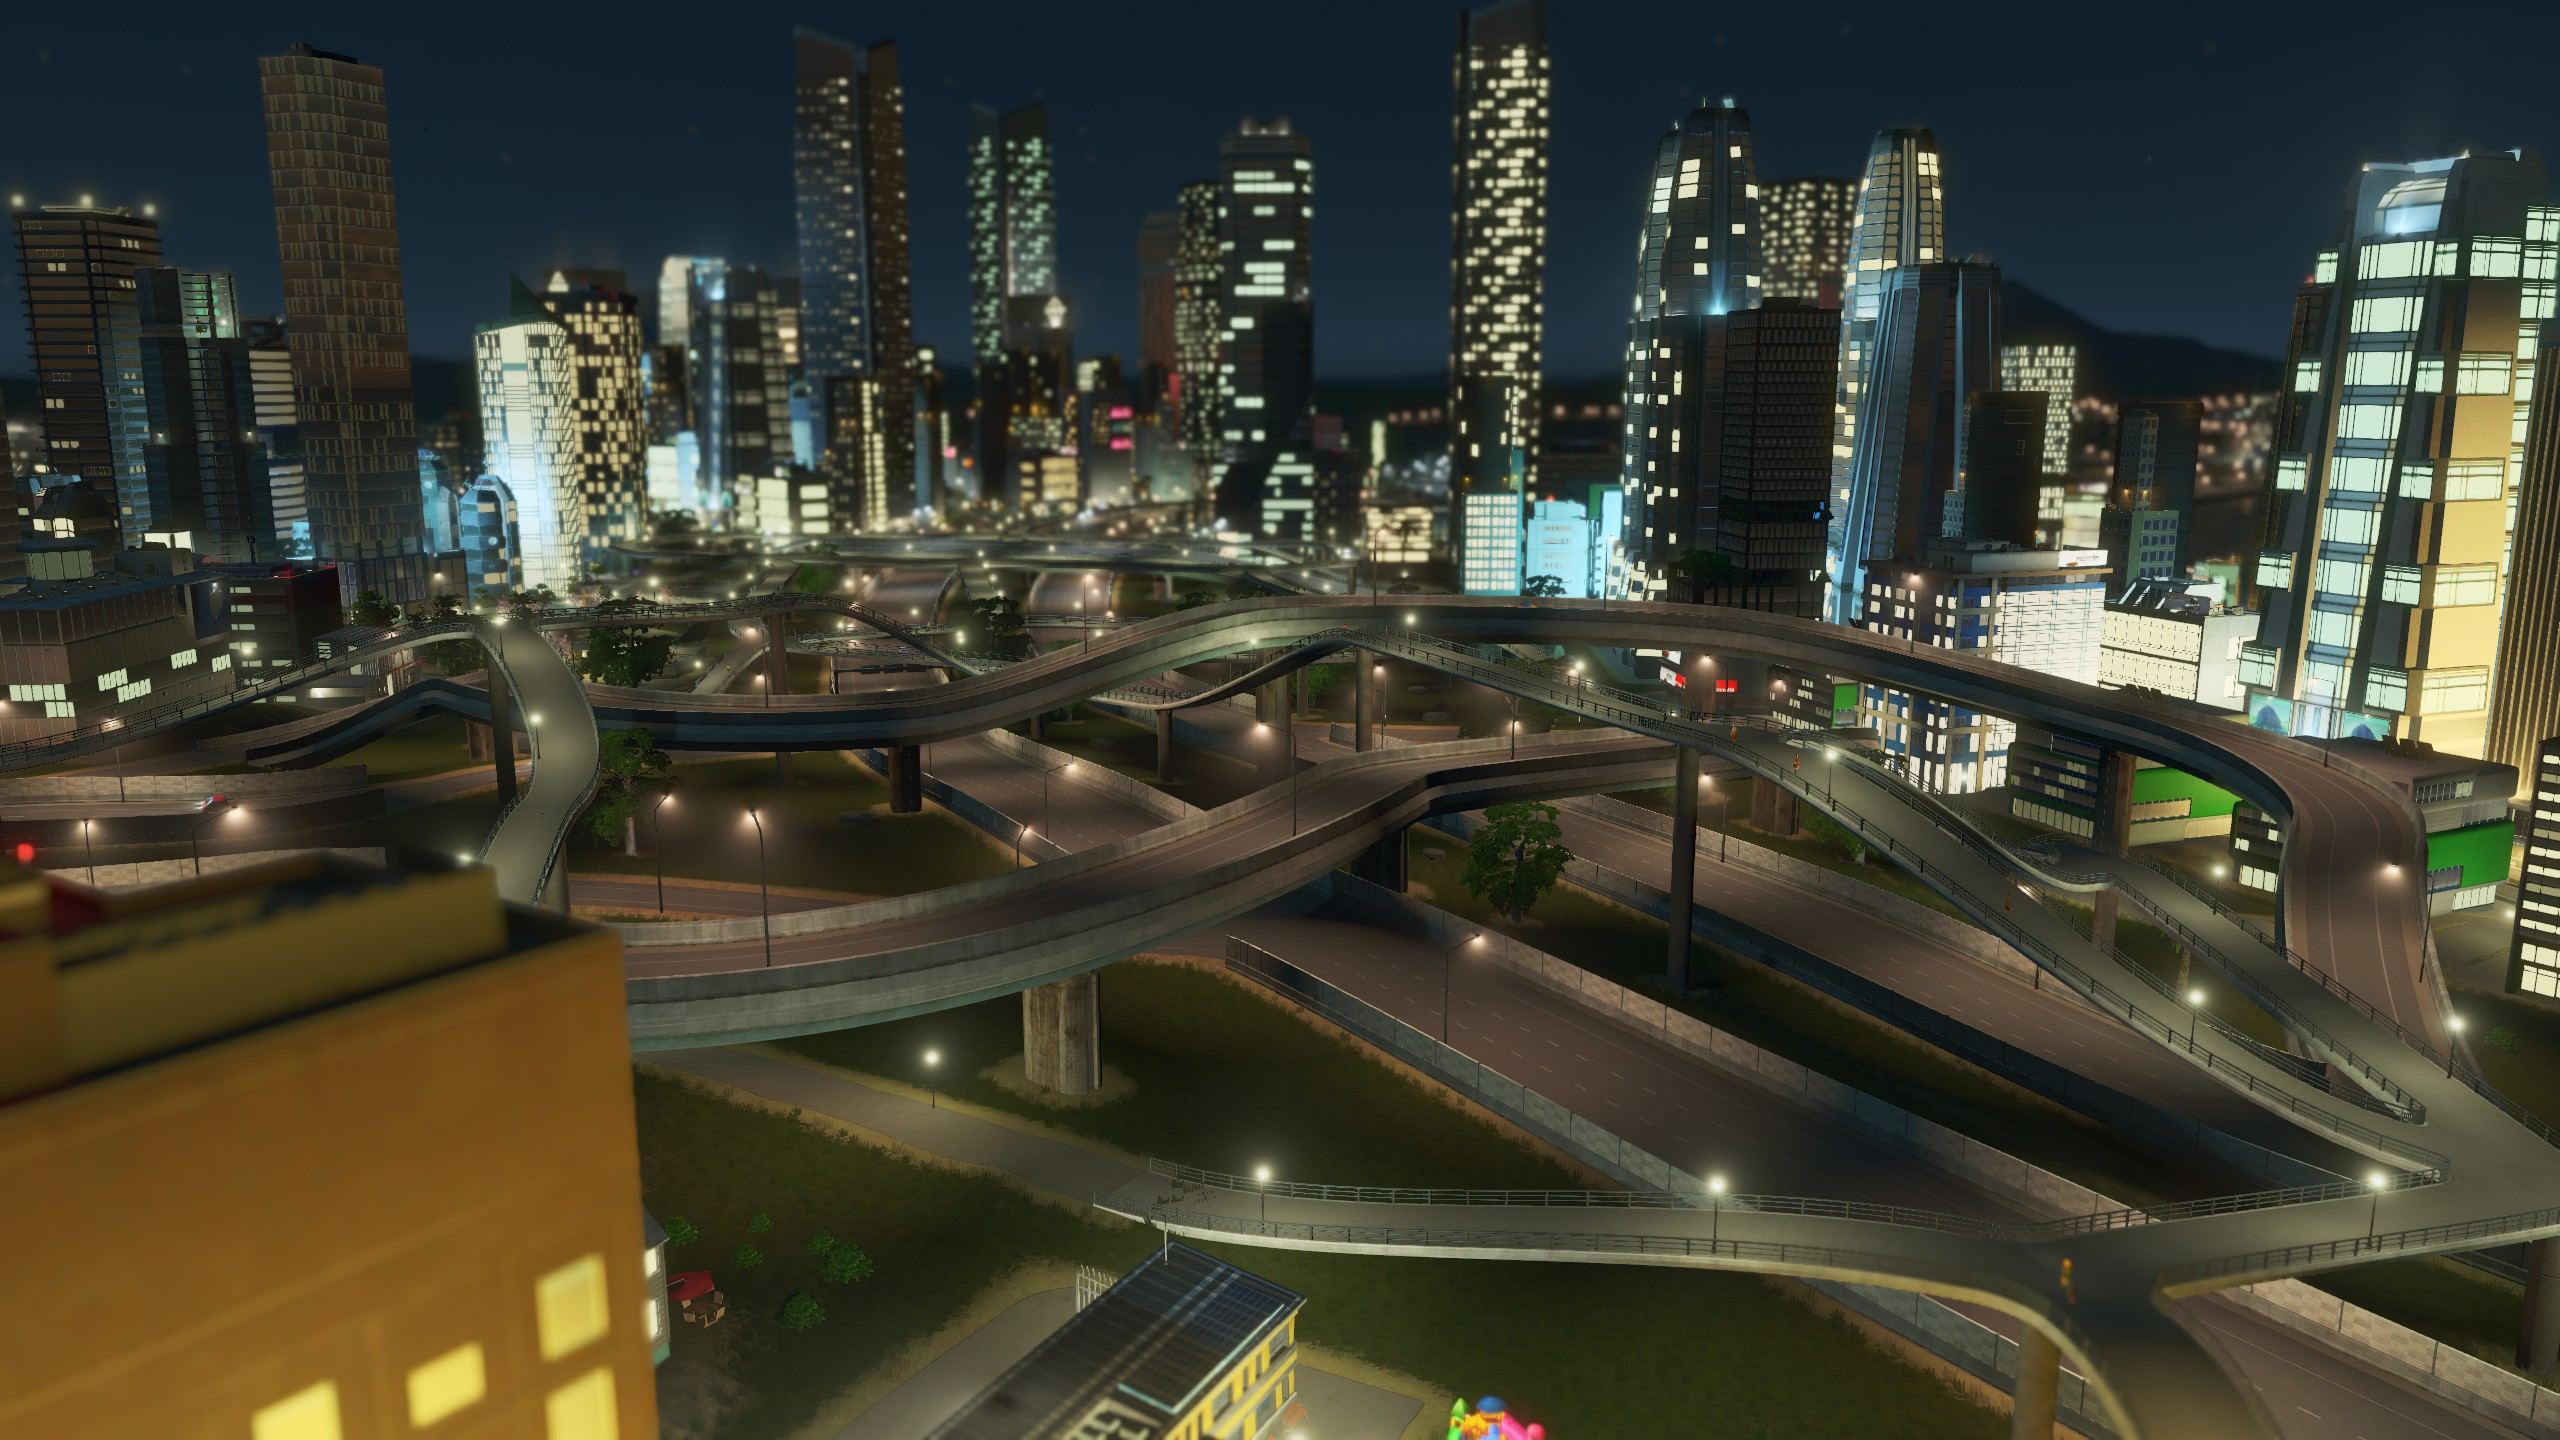
\includegraphics[width=0.6\textwidth]{./figs/fig1-01}
        \caption{TEST FIGURE}
    \end{figure}

\end{spacing}
